\documentclass[10pt]{beamer}

\usetheme[progressbar=frametitle]{metropolis}
\usepackage{appendixnumberbeamer}

\usepackage{booktabs}
\usepackage[scale=2]{ccicons}

\usepackage{pgfplots}
\usepgfplotslibrary{dateplot}

\usepackage{biblatex}
  \addbibresource{type_talk.bib}
\usepackage{minted}
\usepackage{svg}
\usepackage{xypic}

\usepackage{xspace}
\newcommand{\themename}{\textbf{\textsc{metropolis}}\xspace}

%\title{PHP's Type System Dissected}
\title{Typage en PHP comment ça fonctionne ?}
%\subtitle{Understanding how PHP's type system works}
\subtitle{Dissection et explication du système de type de PHP}
% \date{\today}
\date{14 Octobre 2022}
\author{George Peter Banyard}
\institute{The PHP Foundation}

% Logo only on title page
%\titlegraphic{\includegraphics[width=.2\textwidth]{forumphp-2022.png}}
\titlegraphic{
    %\includesvg[inkscapelatex=false,width=0.25\columnwidth]{images/php_foundation.svg}
    %\hfill
    % \baselineskip is the "height" of one line (The normal vertical distance between lines in a paragraph.)
    \includesvg[inkscapelatex=false,height=4\baselineskip]{images/conf_logo.svg}
    %%\includegraphics[width=3cm]{forumphp-2022.png}
}
\makeatletter
\setbeamertemplate{title page}{
  \begin{minipage}[b][\paperheight]{\textwidth}
    \vfill%
    \ifx\inserttitle\@empty\else\usebeamertemplate*{title}\fi
    \ifx\insertsubtitle\@empty\else\usebeamertemplate*{subtitle}\fi
    \usebeamertemplate*{title separator}
      \begin{columns}[T,onlytextwidth]
        \column{0.5\textwidth}
            \ifx\beamer@shortauthor\@empty\else\usebeamertemplate*{author}\fi
            \ifx\insertdate\@empty\else\usebeamertemplate*{date}\fi
            \ifx\insertinstitute\@empty\else\usebeamertemplate*{institute}\fi
        \column{0.5\textwidth}
            %\vfill
            \vspace{0.5cm}
            \hfill
            \ifx\inserttitlegraphic\@empty\else\inserttitlegraphic\fi
            %\hfill
            %\vfill
      \end{columns}
    \vfill
    \vspace*{1cm}
  \end{minipage}
}
\makeatother
% Logo on every slide
%\logo{\includegraphics[width=3cm]{forumphp-2022.png}}
\newcommand{\descriptionsize}{Type universel $\top$ :}

\newcommand{\union}{\:\mathrel{|}\:}
\newcommand{\inter}{\mathrel{\&}}
\newcommand{\mif}{\text{ si }}
\newcommand{\subtype}{\mathrel{<:}}
\newcommand{\suptype}{\mathrel{:>}}
\newcommand{\subtypenot}{\ \not\!\!\subtype}
\newcommand{\type}[1]{\texttt{\textbf{#1}}}

\definecolor{AFUP}{HTML}{36a7df}
\definecolor{AFUP_text}{HTML}{1d2241}
\begin{document}

\maketitle

\begin{frame}{À propos de moi}
    
    \begin{columns}[T,onlytextwidth]
        \column{0.5\textwidth}
            \begin{description}
                  \item[Twitter:] @Girgias
                 \item[GitHub:] Girgias
                  \item[Site:] \url{https://gpb.moe}
            \end{description}
            \begin{center}
                \includesvg[inkscapelatex=false,width=0.8\columnwidth]{images/php_foundation.svg}  
            \end{center}
            
        \column{0.5\textwidth}
            \begin{itemize}
                \item A étudié les maths pures
                \item Core dev de PHP financé à temps partiel par \alert{The PHP Foundation}
                \item Mainteneur principal de la documentation FR de PHP
                \item Auteur des RFCs:
                    \begin{itemize}
                        \item Saner Numeric Strings \cite{banyard_saner_2020}
                        \item Pure Intersection Types \cite{banyard_pure_2021}
                        \item DNF Types \cite{banyard_disjunctive_2022}
                        \item Allow null and false as stand-alone types \cite{banyard_allow_2022}
                        \item True type \cite{banyard_add_2022}
                        \item Et d'autres...
                    \end{itemize}
            \end{itemize}
    \end{columns}
\end{frame}

\begin{frame}{Table des matières}
  \setbeamertemplate{section in toc}[sections numbered]
  \tableofcontents%[hideallsubsections]
\end{frame}

%\section[Intro]{Introduction}
%\begin{verbatim}The theme provides sensible defaults to \emph{emphasize} text, \alert{accent} parts or show \textbf{bold} results.\end{verbatim}
%\begin{center}becomes\end{center}

\section{Terminologie et Symboles}

\begin{frame}{Terminologie}
  \begin{quote}
    Un \alert{système de type} est un système logique constitué d'un ensemble de règles qui assigne la propriété appelée un \textbf{type} à chaque "terme" (un mot, phrase, ou autre ensemble de symbole). Généralement les termes sont des constructions diverses d'un programme informatique, tels que les variables, expressions, fonctions, ou modules.
    Un système de type dicte les \textbf{opérations} qui peuvent être réalisées sur un terme. Pour les variables, le système de type détermine les valeurs permissent de ce terme.
    \cite{noauthor_type_2022}
    % Ref https://en.wikipedia.org/wiki/Type_system
  \end{quote}
\end{frame}

\begin{frame}{Terminologie et Symboles}
    Symboles mathématiques :
    \begin{description}[\descriptionsize]
        \item[$\forall$] Pour tout
        \item[$\exists$] Il existe
        \item[$s \in S$] $s$ appartient à $S$
    \end{description}
    
    Relations entre Types :
    \begin{description}[\descriptionsize]
        \item[$U \subtype V$] $U$ est un sous-type de $V$
        \item[$X \suptype Y$] $X$ est un super-type de $Y$
    \end{description}
    Types Fondamentaux :
    \begin{description}[\descriptionsize]
     \item[Type universel $\top$ :] $\forall T, T \subtype \top$
     \item[Type unitaire $()$ :] type qui n'a qu'une seule valeur
     \item[Type vide $\bot$ :] $\forall T, T \suptype \bot$
    \end{description}
\end{frame}

\section{Système de Type de PHP}
\begin{frame}{Système de Type de PHP}
    En PHP un paramètre de fonction, la valeur de retour d'une fonction, ou une propriété d'une classe peut définir un type.

    Les types disponibles sont :
    \begin{itemize}
        \item Types Primitifs
        \item Types définit en espace Utilisateur
        \item Types Littéraux
        \item Type \texttt{\textbf{callable}}
        \item Types Composés
        \item Alias de Type
    \end{itemize}
\end{frame}

\subsection{Types de bases}
\begin{frame}{Types Primitifs}
    \begin{description}[\descriptionsize]
     \item[Type universel] \texttt{\textbf{mixed}} (PHP 8.0)
     \item[Type objet] \texttt{\textbf{object}} (PHP 7.2)
     \item[Type tableau] \texttt{\textbf{array}}
     \item[Types scalaires] \texttt{\textbf{bool}}, \texttt{\textbf{int}}, \texttt{\textbf{float}}, \texttt{\textbf{string}}
     \item[Type unitaire] \texttt{\textbf{null}} (PHP 8.0*)
     \item[Type vide]  \texttt{\textbf{never}} (PHP 8.1)
    \end{description}
    Et un type de retour spécial:
    \begin{description}[\descriptionsize]
     \item[] \texttt{\textbf{void}} (PHP 7.1)
    \end{description}
\end{frame}

%TODO Graph of type hierarchy ?

\begin{frame}{Types définis en espace Utilisateur}
    Aussi appelés \alert{class-types}, ce sont les:
    \begin{description}[\descriptionsize]
        \item [Interfaces]
        \item [Classes]
        \item [Énumérations] (PHP 8.1)
    \end{description}
    
    Types de classe relatifs :
    \begin{description}[\descriptionsize]
        \item [\texttt{\textbf{self}}]
        \item [\texttt{\textbf{parent}}]
        \item [\texttt{\textbf{static}}] (PHP 8.0 en type de retour uniquement)
    \end{description}
\end{frame}
\begin{frame}{Types littéraux}
    Un type littéral est un sous-type concret d'un type, c.à.d. la valeur d'un type.
    \begin{itemize}
        \item \texttt{\textbf{false}} (PHP 8.0*)
        \item \texttt{\textbf{true}} (PHP 8.2)
    \end{itemize}
    \only
    \begin{alertblock}{Attention}
        Il est impossible de définir un type littéral en espace utilisateur.
        Créez une énumération à la place
    \end{alertblock}
\end{frame}
\begin{frame}{Type \texttt{\textbf{callable}}}
    Type qui représente une fonction:
    \begin{itemize}
        \item Une chaîne de caractères: \texttt{"strlen"}
        \item Une paire objet/nom de méthode: \texttt{[\$instance, "method"]}
        \item Un objet qui implémente \texttt{\_\_invoke()}
        \item Une Closure, récupérable avec la syntaxe: \texttt{strlen(...)} (PHP 8.1)
    \end{itemize}

    \begin{alertblock}{Attention}
        Il est impossible de définir une propriété de classe comme \texttt{\textbf{callable}}
    \end{alertblock}
\end{frame}

\subsection{Types composés}
\begin{frame}{Types composés}
    Un type composé est un type formé de plusieurs autres types.
    \begin{description}[Type d'union simple :]
     \item[Type d'intersection :] \texttt{\textbf{A\&B}} (PHP 8.1)
     \item[Type d'union simple :] \texttt{\textbf{T|U}} (PHP 8.0)
     \item[Type FND :] \texttt{\textbf{(X\&Y)|(V\&W)}} (PHP 8.2)
    \end{description}
    \begin{block}{Forme Normale Disjonctive}
        En calcul des propositions, une \alert{Forme Normale Disjonctive} ou \alert{FND} (en anglais, \emph{disjunctive normal form} ou \emph{DNF}) est une normalisation d'une expression logique qui est une disjonction de clauses conjonctives.
        \cite{noauthor_forme_2022}
        % https://fr.wikipedia.org/wiki/Forme_normale_disjonctive
    \end{block}
\end{frame}
\begin{frame}{Alias de type}
    À partir de PHP 8.2, \texttt{\textbf{iterable}} est un alias de type résolu lors de la compilation.

    \begin{displaymath}
        \text{\texttt{iterable}} := \text{\texttt{Traversable}}|\text{\texttt{array}} 
    \end{displaymath}

    Avant c'était un pseudo-type primitif.
    
    \begin{alertblock}{Attention}
        Il est impossible de définir un alias de type en espace utilisateur.
    \end{alertblock}
\end{frame}

\subsection{Implémentation}
\begin{frame}[fragile]{Implémentation: Vérification du type d'une valeur}
    Chaque valeur en PHP est représentée par une \alert{Zval}.
      \begin{columns}[T,onlytextwidth]
        \column{0.5\textwidth}
    \begin{minted}[fontsize=\footnotesize,]{c}
    struct _zval_struct {
      zend_value value;
      union {
        uint32_t type_info;
        struct {
         /* ... */
        } v;
      } u1;
      /* ... */
    };
    \end{minted}
    
        \column{0.5\textwidth}
    \begin{minted}[fontsize=\footnotesize,]{c}
    #define IS_UNDEF          0
    #define IS_NULL           1
    #define IS_FALSE          2
    #define IS_TRUE           3
    #define IS_LONG           4
    #define IS_DOUBLE         5
    #define IS_STRING         6
    #define IS_ARRAY          7
    #define IS_OBJECT         8
    #define IS_RESOURCE       9
    #define IS_REFERENCE     10
    #define IS_CONSTANT_AST  11
    /* ... */
    \end{minted}
      \end{columns}
\end{frame}

\begin{frame}[fragile]{Implémentation: Vérification du type d'un objet}
      \begin{columns}[T,onlytextwidth]
        \column{0.4\textwidth}
        Structure de classe
    \begin{minted}[fontsize=\tiny,]{c}
struct _zend_class_entry {
  char type;
  zend_string *name;
  zend_class_entry *parent;
  uint32_t ce_flags;
  uint32_t num_interfaces;
  zend_class_entry **interfaces;
  /* ... */
};
    \end{minted}
    Implémentation de \texttt{\textbf{instanceof}}
    \begin{minted}[fontsize=\tiny,]{c}
static zend_always_inline bool
instanceof_function(
  const zend_class_entry *instance_ce,
  const zend_class_entry *ce
) {
  return instance_ce == ce
    || instanceof_function_slow(
               instance_ce, ce);
}
    \end{minted}
    
        \column{0.6\textwidth}
    \begin{minted}[fontsize=\tiny,]{c}
ZEND_API bool ZEND_FASTCALL instanceof_function_slow(
  const zend_class_entry *instance_ce, const zend_class_entry *ce)
{
  if (ce->ce_flags & ZEND_ACC_INTERFACE) {
    if (instance_ce->num_interfaces) {
      for (uint32_t i = 0; i < instance_ce->num_interfaces; i++) {
        if (instance_ce->interfaces[i] == ce) {
          return 1;
        }
      }
    }
    return 0;
  } else {
    while (1) {
      instance_ce = instance_ce->parent;
      if (instance_ce == ce) {
        return 1;
      }
      if (instance_ce == NULL) {
        return 0;
      }
    }
  }
}
    \end{minted}
      \end{columns}
\end{frame}
\begin{frame}[fragile]{zend\_type la représentation d'un type en interne}
    Le type d'un paramètre, valeur de retour ou d'une propriété est représenté par un \alert{zend\_type}.
    \begin{columns}[T,onlytextwidth]
        \column{0.5\textwidth}
            \begin{minted}[fontsize=\footnotesize,]{c}
typedef struct {
  void *ptr;
  uint32_t type_mask;
} zend_type;
            \end{minted}
            \texttt{\textbf{ptr}} est soit une classe sous forme de chaîne
            soit une liste \\de type:
            \begin{minted}[fontsize=\footnotesize,]{c}
typedef struct {
  uint32_t num_types;
  zend_type types[1];
} zend_type_list;
            \end{minted}
    
        \column{0.5\textwidth}
            Masque de bit pour les types primitifs
            \begin{minted}[fontsize=\tiny,breaklines,breakafter=|]{c}
#define MAY_BE_UNDEF     (1 << IS_UNDEF)
#define MAY_BE_NULL      (1 << IS_NULL)
#define MAY_BE_FALSE     (1 << IS_FALSE)
#define MAY_BE_TRUE      (1 << IS_TRUE)
#define MAY_BE_BOOL      (MAY_BE_FALSE|MAY_BE_TRUE)
#define MAY_BE_LONG      (1 << IS_LONG)
#define MAY_BE_DOUBLE    (1 << IS_DOUBLE)
#define MAY_BE_STRING    (1 << IS_STRING)
#define MAY_BE_ARRAY     (1 << IS_ARRAY)
#define MAY_BE_OBJECT    (1 << IS_OBJECT)
#define MAY_BE_RESOURCE  (1 << IS_RESOURCE)
#define MAY_BE_ANY       (MAY_BE_NULL|MAY_BE_FALSE|MAY_BE_TRUE|MAY_BE_LONG|MAY_BE_DOUBLE|MAY_BE_STRING|MAY_BE_ARRAY|MAY_BE_OBJECT|MAY_BE_RESOURCE)
#define MAY_BE_CALLABLE  (1 << IS_CALLABLE)
#define MAY_BE_VOID      (1 << IS_VOID)
#define MAY_BE_NEVER     (1 << IS_NEVER)
#define MAY_BE_STATIC    (1 << IS_STATIC)
            \end{minted}
    \end{columns}
\end{frame}

\section{Héritage et Principe de Substitution de Liskov}
\begin{frame}{Principe de Substitution de Liskov}
    Le principe de substitution de Liskov (en anglais \emph{Liskov Substitution Principle} ou \alert{LSP}) est, en programmation orientée objet, une définition particulière de la notion de sous-type. Il a été formulé par Barbara Liskov et Jeannette Wing en 1993. \cite{liskov_behavioral_1994}
    
    La formulation condensée est:
    \begin{quote}
        Si $\mathbf{\phi(x)}$ est une propriété démontrable pour tout objet $\mathbf{x}$ de type $\mathbf{T}$, alors $\mathbf{\phi(y)}$ est vraie pour tout objet $\mathbf{y}$ de type $\mathbf{S}$ tel que $\mathbf{S}$ est un sous-type de $\mathbf{T}$
        
        %Cite https://dl.acm.org/doi/10.1145/197320.197383
    \end{quote}
\end{frame}
\begin{frame}{Principe de Substitution de Liskov: Simplifié}
    LSP est un principe à propos du remplacement d'un type par un autre tel que les interactions avant et après ne soient pas perturbées.

    \begin{description}
        \item[Les pré-conditions] ne peuvent pas être renforcées dans une sous-type
        \item[Les post-conditions] ne peuvent pas être affaiblies dans un sous-type
        \item[Les invariants] doivent être conservé dans un sous-type
    \end{description}
\end{frame}
\begin{frame}{Principe de Substitution de Liskov: Simplifié}
    \begin{figure}
    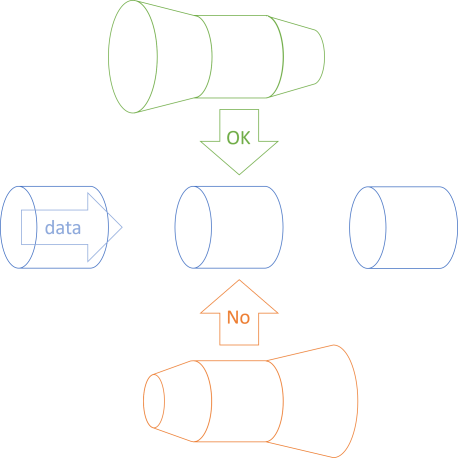
\includegraphics{lsp-pipes.png}
    \caption{
        Visualisation du Principe du Substitution de Liskov comme un tuyau. \cite{seemann_liskov_2021}
    }
        %Source: \href{https://blog.ploeh.dk/2021/12/06/the-liskov-substitution-principle-as-a-profunctor/}
        %{The Liskov Substitution Principle as a profunctor by Mark Seemann}
        %\cite{knuth92,ConcreteMath,Simpson,Er01,greenwade93}
  \end{figure}
\end{frame}
\begin{frame}{Effet de LSP sur les signatures}
    \begin{description}
        \item[Les méthodes] ne peuvent pas ajouter de paramètres obligatoires.
        \item[Le type des paramètres] des méthodes doit être \emph{contra-variant},\\c.à.d. un super-type.
        \item[Le type de retour] des méthodes doit être \emph{co-variant},\\c.à.d. un sous-type.
        \item[Le type des propriétés] doit être \emph{co} \textbf{et} \emph{contra-variant}.
    \end{description}
\end{frame}

\subsection{Implémentation}
\begin{frame}[fragile]{Implémentation}
    Pour la vérification de la compatibilité des types on a juste besoin de:
%\begingroup \fontsize{1pt}{1pt}\selectfont \endgroup
    \begin{minted}[fontsize=\footnotesize,breaklines]{c}
static inheritance_status zend_perform_covariant_type_check(
    zend_class_entry *fe_scope, zend_type fe_type,
    zend_class_entry *proto_scope, zend_type proto_type)
{
    /* ... */
}
    \end{minted}
    où \texttt{fe} représente le sous-type, et \texttt{proto} le super-type
\end{frame}
\begin{frame}[fragile]{Implémentation: covariance de types primitifs}
%\begingroup \fontsize{1pt}{1pt}\selectfont \endgroup
    \begin{minted}[fontsize=\tiny,breaklines]{c}
/* Apart from void, everything is trivially covariant to the mixed type.
 * Handle this case separately to ensure it never requires class loading. */
if (ZEND_TYPE_PURE_MASK(proto_type) == MAY_BE_ANY &&
        !ZEND_TYPE_CONTAINS_CODE(fe_type, IS_VOID)) {
    return INHERITANCE_SUCCESS;
}

/* Builtin types may be removed, but not added */
uint32_t fe_type_mask = ZEND_TYPE_PURE_MASK(fe_type);
uint32_t proto_type_mask = ZEND_TYPE_PURE_MASK(proto_type);
uint32_t added_types = fe_type_mask & ~proto_type_mask;
if (added_types) {
    if ((added_types & MAY_BE_STATIC) &&
            zend_type_permits_self(proto_type, proto_scope, fe_scope)) {
        /* Replacing type that accepts self with static is okay */
        added_types &= ~MAY_BE_STATIC;
    }
    if (added_types == MAY_BE_NEVER) {
        /* never is the bottom type */
        return INHERITANCE_SUCCESS;
    }
    if (added_types) {
        /* Otherwise adding new types is illegal */
        return INHERITANCE_ERROR;
    }
}
    \end{minted}
\end{frame}

\begin{frame}{$U$ un type d'union, est ce que $U \subtype V$ ?}
    $U_i \in U$, $V_j \in V$
    \begin{align}
        \mif\forall U_i, \exists V_j : U_i \subtype V_j & \implies U_1\union\cdots\union U_n \subtype V_1\union\cdots\union V_m \\
        \mif\forall U_i, \forall V_j : U_i \subtype V_j & \implies U_1\union\cdots\union U_n \subtype V_1\inter\cdots\inter V_m
    \end{align}
    On doit itérer sur l'ensemble de type $U$ d'abord, et juste vérifier si chaque $U_i$ est un sous-type de $V$. 
\end{frame}
\begin{frame}[fragile]{Implémentation: $U$ un type d'union, est-ce que $U \subtype V$ ?}
%\begingroup \fontsize{1pt}{1pt}\selectfont \endgroup
    \begin{minted}[fontsize=\tiny,breaklines]{c}
early_exit_status = INHERITANCE_ERROR;
ZEND_TYPE_FOREACH(fe_type, single_type) {
    inheritance_status status;
    /* Union has an intersection type as it's member */
    if (ZEND_TYPE_IS_INTERSECTION(*single_type)) {
        status = zend_is_intersection_subtype_of_type(
            fe_scope, *single_type, proto_scope, proto_type);
    } else {
        zend_string *fe_class_name = get_class_from_type(fe_scope, *single_type);
        if (!fe_class_name) {
            continue;
        }

        status = zend_is_class_subtype_of_type(
            fe_scope, fe_class_name, proto_scope, proto_type);
    }

    if (status == early_exit_status) {
        return status;
    }
} ZEND_TYPE_FOREACH_END();
    \end{minted}
\end{frame}

\begin{frame}{$U$ un type d'intersection, est-ce que $U \subtype V$ ?}
    Un type d'intersection en PHP est forcément un objet, donc si \texttt{object} $\in V$ alors $U \subtype V$.

    Dans le cas général:
    $U_i \in U$, $V_j \in V$
    \begin{align}
        \mif\exists V_j, \exists U_i : U_i \subtype V_j & \implies U_1\inter\cdots\inter U_n \subtype V_1\union\cdots\union V_m \\
        \mif\forall V_j, \exists U_i : U_i \subtype V_j & \implies U_1\inter\cdots\inter U_n \subtype V_1\inter\cdots\inter V_m
    \end{align}

    Comme l'\emph{ordre} des quantificateurs est inversé comparé au cas d'un type d'union, on doit d'abord itérer sur $V$.
    Si $V$ est un type d'union, il suffit d'une seule paire $(i;j)$ qui satisfait  $U_i \subtype V_j$ pour que $U \subtype V$.
    Dans le cas contraire il faut que chaque $V_j$ soit satisfait par au moins un $U_i$ pour que $U \subtype V$.
\end{frame}
\begin{frame}[fragile]{Implémentation: $U$ un type d'intersection, est ce que $U \subtype V$ ?}
%\begingroup \fontsize{1pt}{1pt}\selectfont \endgroup
    \begin{minted}[fontsize=\tiny,breaklines]{c}
static inheritance_status zend_is_intersection_subtype_of_type(
    zend_class_entry *fe_scope, zend_type fe_type,
    zend_class_entry *proto_scope, zend_type proto_type)
{
    inheritance_status early_exit_status =
        ZEND_TYPE_IS_INTERSECTION(proto_type) ? INHERITANCE_ERROR : INHERITANCE_SUCCESS;
    ZEND_TYPE_FOREACH(proto_type, single_type) {
        inheritance_status status;

        if (ZEND_TYPE_IS_INTERSECTION(*single_type)) {
            status = zend_is_intersection_subtype_of_type(
               fe_scope, fe_type, proto_scope, *single_type);
        } else {
            zend_string *proto_class_name = get_class_from_type(proto_scope, *single_type);
            if (!proto_class_name) {
                continue;
            }

            zend_class_entry *proto_ce = NULL;
            status = zend_is_intersection_subtype_of_class(
                fe_scope, fe_type, proto_scope, proto_class_name, proto_ce);
        }

        if (status == early_exit_status) {
            return status;
        }
    } ZEND_TYPE_FOREACH_END();
    return early_exit_status == INHERITANCE_ERROR ? INHERITANCE_SUCCESS : INHERITANCE_ERROR;
}
    \end{minted}
\end{frame}

\section{Le futur?}
\begin{frame}[fragile]{Le futur?}
    \begin{description}
        \item Alias de type en espace utilisateur
            \begin{minted}[fontsize=\scriptsize,breaklines]{php}
typedef numeric int|float
            \end{minted}
        \item Type de fonction
            \begin{minted}[fontsize=\scriptsize,breaklines]{php}
foo(fn<int,string>:bool $callable) {} 
            \end{minted}
        \item Type générique
            \begin{minted}[fontsize=\scriptsize,breaklines]{php}
class Collection<T> {
    private array<T> $stack = [];
    public function add(T $v) {
        $this->stack[] $v;
    }
}
            \end{minted}
        \item Paramètres \texttt{in-out}
            \begin{minted}[fontsize=\scriptsize,breaklines]{php}
function foo(inout array $v) { $v = 5; }
$a = [];
foo($a); // TypeError: inout argument 1 passed to foo() must be of the type array, int assigned
            \end{minted}
    \end{description}
\end{frame}


{\setbeamercolor{palette primary}{fg=AFUP_text, bg=AFUP}
\begin{frame}[standout]
    Merci beaucoup!
    \vfill
    \begin{columns}[T,onlytextwidth]
        \column{0.5\textwidth}
            \begin{center}
                \begin{description}
                    \item[Twitter:] @Girgias
                    \item[GitHub:] Girgias
                    \item[Site:] \url{https://gpb.moe}
                \end{description}
            \end{center}
        \column{0.5\textwidth}
            \begin{center}
                Feedback:
                
                \vspace{0.5cm}
                
\includegraphics[width=3cm]{images/Forum_PHP_2022_QRCode.png}
            \end{center}
    \end{columns}
\end{frame}
}

\appendix


\begin{frame}[fragile]{Coercitions de types scalaire}
    Par défaut PHP coerce les valeurs scalaires vers un type scalaire autorisé.
    S'il y a plusieurs types scalaires alors l'ordre est le suivant :
    \begin{enumerate}
        \item \type{int}
        \item \type{float}
        \item \type{string}
        \item \type{bool}
    \end{enumerate}
    \begin{exampleblock}{Note}
       Si la valeur est une \type{string} et le type déclaré a \type{int} et \type{float} alors la sémantique de chaînes numérique décide du type de destination.
    \end{exampleblock}
    \begin{exampleblock}{Note}
        Les fonctions internes coerce \type{null}, obsolète à partir de PHP 8.1.
    \end{exampleblock}
\end{frame}

\begin{frame}[fragile]{\texttt{strict\_types}}
    Que fait \texttt{strict\_types} ?
    \pause
    
    Plus de coercitions pour les types scalaires dans les cas suivant \alert{uniquement} :
    \begin{itemize}
        \item Appel de fonction dans le fichier qui définit \texttt{strict\_types}
        \item Valeur de retour pour une fonction définit en espace utilisateur
        \item Assignation de valeur à une propriété typé
    \end{itemize}
\end{frame}
\begin{frame}[fragile]{\texttt{strict\_types}}
    \texttt{strict\_types} ne change \alert{pas} le comportement :

    \begin{itemize}
        \item Des opérateurs binaires:
            \begin{minted}[fontsize=\scriptsize,breaklines]{php}
<?php
declare(strict_types=1);
var_dump(10 + "45"); // int(55)
var_dump(true . " hello"); // string(7) "1 hello"
            \end{minted}
        \item Des opérateurs de comparaison
            \begin{minted}[fontsize=\scriptsize,breaklines]{php}
<?php
declare(strict_types=1);
var_dump("1" == "01"); // bool(true)
var_dump(014 == "14"); // bool(false)
var_dump(14 == "014"); // bool(true)
            \end{minted}
        \item Des constructions de langages
            \begin{minted}[fontsize=\scriptsize,breaklines]{php}
<?php
declare(strict_types=1);
exit(true); // Écrira "1" et non pas un code de sortie 1 comme si exit(1) aurait été utilisé
            \end{minted}
    \end{itemize}
\end{frame}
\begin{frame}[fragile]{\texttt{strict\_types}}
    \texttt{strict\_types} ne change \alert{pas} le comportement :

    \begin{itemize}
        \item De la coercitions des types scalaires pour les fonctions appelées par le moteur
            \begin{minted}[fontsize=\scriptsize,breaklines]{php}
<?php
declare(strict_types=1);
$f = fn (int $i): bool => (bool) ($i % 2);
$a = ['1', '2', 3, 4, '5.0', '6.0'];
var_dump(array_filter($a, $f));
            \end{minted}
            Résultat :
            \begin{minted}[fontsize=\scriptsize,breaklines]{php}
array(3) {
  [0]=>
  string(1) "1"
  [2]=>
  int(3)
  [4]=>
  string(3) "5.0"
}
            \end{minted}
    \end{itemize}
\end{frame}

\begin{frame}[fragile]{Exemples LSP}
    \begin{columns}[T,onlytextwidth]
        \column{0.5\textwidth}
    \begin{minted}[fontsize=\scriptsize,breaklines]{php}
<?php
interface I {}
class U implements I {}
class V implements I {}

class Super {
    public function foo(): I {}
}
class Sub extends Super {
    public function foo(): U|V {}
}
    \end{minted}
        \column{0.5\textwidth}
    \begin{minted}[fontsize=\scriptsize,breaklines]{php}
<?php
interface A {}
interface B {}
class X implements A, B {}
class Y implements A, B {}

class Super {
    public function foo(): A&B {}
}
class Sub extends Super {
    public function foo(): X|Y {}
}
    \end{minted}
    \end{columns}
\end{frame}

\begin{frame}[allowframebreaks]{References}

  %\bibliography{type_talk}
  %\bibliographystyle{abbrv}
  \printbibliography

\end{frame}

\end{document}
